\documentclass[12pt,a4paper]{article}
\usepackage[UTF8]{ctex}
\usepackage{geometry}
\usepackage{graphicx}
\usepackage{float}
\usepackage{amsmath}
\usepackage{amsfonts}
\usepackage{amssymb}
\usepackage{booktabs}
\usepackage{multirow}
\usepackage{array}
\usepackage{longtable}
\usepackage{enumerate}
\usepackage{fancyhdr}
\usepackage{lastpage}
\usepackage{hyperref}
\usepackage[normalem]{ulem}


% 页面设置
\geometry{left=2.5cm,right=2.5cm,top=2.5cm,bottom=2.5cm}
\setlength{\headheight}{15pt}

% 页眉页脚设置
\pagestyle{fancy}
\fancyhf{}
\fancyhead[C]{实\hspace{0.5em}验\hspace{0.5em}原\hspace{0.5em}始\hspace{0.5em}记\hspace{0.5em}录}
\fancyfoot[L]{\parbox[t]{\textwidth}{实验人员：\underline{陈恪瑾}  学号：\underline{U202413925}  同组人员：\underline{黄伟峰}}}
\fancyfoot[R]{教师签字：\underline{\hspace{3cm}}}

\begin{document}

% 正文第一行标题
\noindent
{\Large \textbf{实验八：}\underline{\textbf{元件特性的示波器测量法}}} \hfill {\Large \textbf{实验台编号：}\underline{\textbf{05}}}
\vspace{0.5cm}

\section*{一、实验注意事项}
\begin{enumerate}
    \item 测量中，信号发生器作为信号源，示波器作为测量仪器，它们的公共接地必须与电路中的"地"端连接在一处。
    \item 测量中，在选择电源时，应从小到大逐步调节，以测量出完整的特性曲线。
    \item 电路连接或拆线时，要先关闭信号源。
\end{enumerate}

\section*{二、实验线路}
\begin{figure}[H]
    \centering
    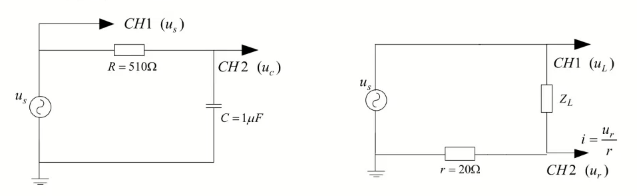
\includegraphics[width=0.8\textwidth]{templete_preview/1.png}
    \caption{RC电路相位差测量电路图}
    \label{fig:circuit}
\end{figure}



\section*{三、拍照记录}
\begin{enumerate}
    \item 移相电路相位差的测量。
    

    
    \item 测量510$\Omega$电阻的伏安特性曲线，以及幅值图形显示。
    \item 测量非线性电阻元件的特性曲线（X-Y模式）。
\end{enumerate}

\end{document}
